\chapter{Testowanie Contiguous Memory Allocatora}

Aby sprawdzić działanie alokatora \acc{CMA}, w~tym rozdziale opiszę
jak go przetestować na przykładzie laptopa \acc{MSI} U100 z~jednym
\unit{GiB} pamięci \acc{RAM} z~zainstalowanym systemem Slackware 14.0.
Do testów wybrałem tę dystrybucję \acc{GNU}/Linuksa, gdyż jest ona
stosunkowo prosta w~użyciu, a~jednocześnie pozostaje wierny filozofii
Uniksa, dzięki czemu łatwo jest wymieniać komponenty systemu takie jak
jądro.


\section{Instalacja jądra z~obsługą \acc{CMA}}

Standardowo Linux nie posiada obsługi alokatora \acc{CMA}, dlatego pierwszym
krokiem będzie zmiana jądra systemu na Linux 3.5 z~włączonym
mechanizmem \acc{CMA}.  Źródła można pobrać ze strony
\url{http://kernel.org/}, która jest głównym miejscem dystrybucji
Linuksa.

Przed kompilacją jądra należy najpierw je skonfigurować.  Aby ułatwić
ten proces, zamiast ustawiać wszystko od początku, warto skorzystać
z~już istniejącego pliku konfiguracyjnego.  Zazwyczaj konfiguracja
obecnie uruchomionego jądra jest dostępna w~pliku
\code{/proc/config.gz}.  Aby uruchomić program konfiguracji jądra,
należy wykonać następującą sekwencję poleceń:

\begin{lstlisting}[language=sh,numbers=none]
wget http://www.kernel.org/pub/linux/kernel/v3.0/linux-3.5.tar.xz
xz -d <linux-3.5.tar.xz | tar xf
cd linux-3.5
gzip -d </proc/config.gz >.config
make xconfig
\end{lstlisting}

Uruchomi to graficzny interfejs użytkownika\footnote{W~przypadku
  kompilacji w~środowisku tekstowym, zamiast polecenia \code{make
    xconfig} należy wykonać komendę \code{make menuconfig}, które
  uruchomi interfejs tekstowy oparty o~bibliotekę ncurses.}, który
pozwala wybrać opcje z~jakimi jądro ma zostać zbudowane.  Aby móc
testować \acc{CMA} należy w~nim zaznaczyć opcje \ang*{Prompt for development
  and/or incomplete code/drivers} w~sekcji \ang*{General setup}
(zob.\ rysunek \subref*{fig:xconfig-exp}) oraz \ang*{Contiguous Memory
  Allocator} w~sekcji \ang*{Device Drivers $\rightarrow$ Generic
  Driver Options} (zob.\ rysunek \subref*{fig:xconfig-cma}).  Ponadto,
aby umożliwić dalsze testy należy również upewnić się, że opcja
\ang*{Enable loadable module support} jest wybrana.

\begin{figure}[tbp]
  \centering
  \subfloat[Opcja umożliwiająca wybór eksperymentalnych funkcji jądra.]{
    \label{fig:xconfig-exp}
    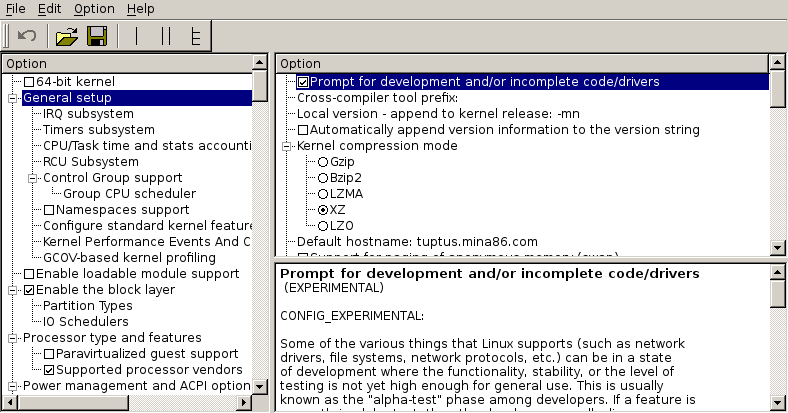
\includegraphics[width=.9\textwidth]{build/xconfig-exp.eps}
  } \\
  \subfloat[Opcja włączająca \acc{CMA}.]{
    \label{fig:xconfig-cma}
    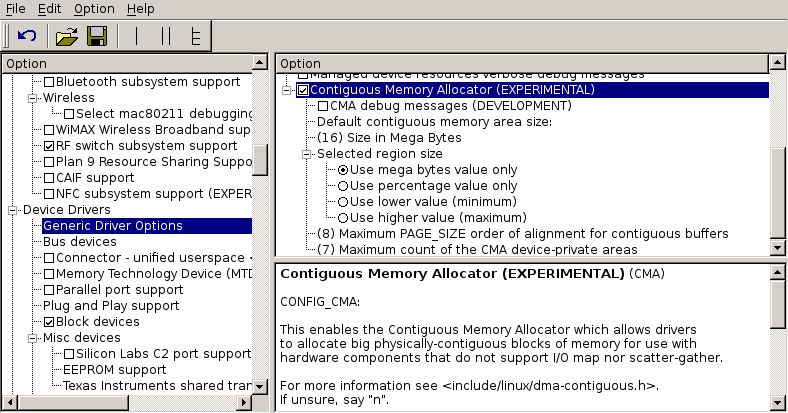
\includegraphics[width=.9\textwidth]{build/xconfig-cma.eps}
  }
  \caption{Graficzny interfejs konfiguracji jądra.}
  \label{fig:xconfig}
\end{figure}

Gdy konfiguracja zostanie zakończenie należy zbudować i~zainstalować
nowe jądro zgodnie z~opisem w~\autocite{bib:building-linux}.  Aby móc
testować alokator \acc{CMA}, należy stworzyć dodatkowe wpisy
w~\code{/etc/lilo.conf} różniące się opcją \code{append} (która
powoduje, że program startujący przekazuje dodatkowe opcje do jądra):

\begin{itemize}
\item \code{append = "cma=0"} wyłączy \acc{CMA} tak, że jądro będzie
  zachowywać się jakby obsługa \acc{CMA} nie była dostępna w~jądrze.
\item \code{append = "cma=0 mem=512m"} spowoduje, że Linux będzie
  korzystał tylko z~pierwszych \unit[512]{MiB} pamięci \acc{RAM}.  Ustawienie
  to pozwala symulować sytuację, w~której część pamięci jest na stałe
  zarezerwowane dla sterowników.
\item \code{append = "cma=512m"} skonfiguruje alokator \acc{CMA}, tak aby
  zarezerwował pojedynczy region rozmiaru \unit[512]{MiB} do
  wykorzystania dla sterowników.
\end{itemize}

Po uruchomieniu nowego jądra, obecność mechanizmu \acc{CMA} można sprawdzić
analizując plik \code{/proc/pagetypeinfo}.  Zawiera on statystyki
alokatora stron w~postaci liczby ramek różnych typów w~poszczególnych
strefach.  Ponadto plik \code{/proc/cmdline} zawiera pełną listę
argumentów jakie program startujący przekazał jądru, może on być
przydatny do weryfikacji, czy opcje są poprawnie przekazywane.


\section{Testowanie alokacji pamięci}

Aby zobaczyć efekt działania opcji \code{mem} wykorzystać można prosty
program \code{malloc} przedstawiony na wydruku \ref{lst:malloc}.  Nie
robi on nic poza alokacją pamięci w~pętli aż do momentu, gdy zabraknie
pamięci w~systemie.  Linux domyślnie opóźnia alokację pamięci aż do
próby pierwszej modyfikacji dlatego program musi zapisać wartość jeden
w~zaalokowanej stronie.

\begin{lstlisting}[float=tb,caption=Prosty program testujący alokację
    pamięci.,label=lst:malloc]
#include <stdlib.h>
#include <stdio.h>

int main(void) {
	long i = 0;
	while (1) {
		printf("\r%10ld", ++i * 4);
		fflush(stdout);
		*(char *)malloc(4096) = '1';
	}
}
\end{lstlisting}

Gdy jądro nie będzie już w~stanie zaspokoić żądań alokacji pamięci
programu, \ang*{out-of-memory killer} wymusi jego zakończenie.  Jest
to mechanizm jądra, którego celem jest zagwarantowanie, iż system
zawsze będzie miał pewne rezerwy wolnej pamięci.

Uruchomiony na testowym systemie z~jednym \unit{GiB} zakończył się
przy próbie alokacji \unit[988\,284]{KiB}, gdy \acc{CMA} był
wyłączony, oraz \unit[987\,628]{KiB}, gdy \acc{CMA} był
skonfigurowany, aby zarezerwować region o~rozmiarze \unit[512]{MiB}.
Różnica jednego megabajta jest pomijalna i~wskazuje, iż istotnie
pamięć rezerwowana przez \acc{CMA} jest dostępna dla systemu.

Jednocześnie gdy jądro zostanie uruchomione z~opcją \code{mem=512m},
program został zatrzymany przy próbie alokacji \unit[488\,900]{KiB}.
Pokazuje to w~praktyce działanie argumentu \code{mem} jądra.


\section{Modułu testowy cma\_test}

Do testów \acc{CMA} wykorzystam moduł Barry'ego Songa
\autocite{patch:cma-test}.  Po nałożeniu do źródeł jądra 3.5 stworzy
on nowy katalog \code{tools/cma} z~testowym sterownikiem.  Był on
testowany na architekturze \acc{ARM} i~aby zadziałał na systemie x86 należy
zmodyfikować plik \code{cma_test.c} wprowadzając dwie zmiany.  Po
pierwsze, zaraz po ostatniej dyrektywie \code{#include} należy dodać
następujące linie:

\begin{lstlisting}
#ifndef SZ_1K
#  define SZ_1K 1024
#endif

static u64 cma_test_dma_mask = ~(u64)0;
\end{lstlisting}

Po wtóre, w~funkcji \code{cma_test_init}, tuż przed linią przypisującą
wartość do pola \code{coherent_dma_mask} obiektu \code{cma_dev},
należy dodać linijkę:

\begin{lstlisting}
	cma_dev->dma_mask = &cma_test_dma_mask;
\end{lstlisting}

Po wprowadzeniu tych modyfikacji moduł można skompilować wykonując
polecenie \code{make} wewnątrz katalogu \code{tools/cma}, co spowoduje
utworzenie pliku \code{cma_test.ko}.

Po wczytaniu tego modułu poleceniem \code{insmod cma_test.ko}
w~systemie pojawi się urządzenie \code{/dev/cma_test}, które służy do
wykonywania testowych alokacji z~wykorzystaniem interfejsu \acc{DMA} \acc{API}
(a~zatem pośrednio z~użyciem alokatora \acc{CMA}).  Zapis do tego pliku
liczby naturalnej spowoduje wykonanie alokacji podanej liczby
kibibajtów, a~odczyt zwolnienie najwcześniej zaalokowanego obszaru.

Przykładowo, po wykonaniu polecenia \code{echo 524288 >/dev/cma_test}
połowa pamięci systemu zostanie przydzielona sterownikowi
\code{cma_test}.  Można to potwierdzić uruchamiając ponownie program
\code{malloc}, który zostanie zatrzymany po zaalokowaniu niecałych
\unit[500]{MiB}.
